\documentclass{warpdoc}
\newlength\lengthfigure                  % declare a figure width unit
\setlength\lengthfigure{0.158\textwidth} % make the figure width unit scale with the textwidth
\usepackage{psfrag}         % use it to substitute a string in a eps figure
\usepackage{subfigure}
\usepackage{rotating}
\usepackage{pstricks}
\usepackage[innercaption]{sidecap} % the cute space-saving side captions
\usepackage{scalefnt}
\usepackage{bm}
\usepackage{amsmath}

%%%%%%%%%%%%%=--NEW COMMANDS BEGINS--=%%%%%%%%%%%%%%%%%%%%%%%%%%%%%%%%%%
\newcommand{\alb}{\vspace{0.2cm}\\} % array line break
\newcommand{\rhos}{\rho}
\newcommand{\Cv}{{C_{\rm v}}}
\newcommand{\Cp}{{C_{\rm p}}}
\newcommand{\Sct}{{{\rm Sc}_{\rm T}}}
\newcommand{\Prt}{{{\rm Pr}_{\rm T}}}
\newcommand{\nd}{{{n}_{\rm d}}}
\newcommand{\ns}{{{n}_{\rm s}}}
\newcommand{\nn}{{{n}_{\rm n}}}
\newcommand{\ndm}{{\bar{n}_{\rm d}}}
\newcommand{\nsm}{{\bar{n}_{\rm s}}}
\newcommand{\turb}{_{\rm T}}
\newcommand{\mut}{{\mu\turb}}
\newcommand{\mfa}{\scriptscriptstyle}
\newcommand{\mfb}{\scriptstyle}
\newcommand{\mfc}{\textstyle}
\newcommand{\mfd}{\displaystyle}
\newcommand{\hlinex}{\vspace{-0.34cm}~~\\ \hline \vspace{-0.31cm}~~\\}
\newcommand{\hlinextop}{\vspace{-0.46cm}~~\\ \hline \hline \vspace{-0.32cm}~~\\}
\newcommand{\hlinexbot}{\vspace{-0.37cm}~~\\ \hline \hline \vspace{-0.50cm}~~\\}
\newcommand{\tablespacing}{\vspace{-0.4cm}}
\newcommand{\fontxfig}{\footnotesize\scalefont{0.918}}
\newcommand{\fontgnu}{\footnotesize\scalefont{0.896}}
\renewcommand{\fontsizetable}{\footnotesize\scalefont{1.0}}
\renewcommand{\fontsizefigure}{\footnotesize}
\renewcommand{\vec}[1]{\bm{#1}}
\setcounter{tocdepth}{3}
\let\citen\cite

%%%%%%%%%%%%%=--NEW COMMANDS BEGINS--=%%%%%%%%%%%%%%%%%%%%%%%%%%%%%%%%%%

\setcounter{tocdepth}{3}

%%%%%%%%%%%%%=--NEW COMMANDS ENDS--=%%%%%%%%%%%%%%%%%%%%%%%%%%%%%%%%%%%%



\author{
  Bernard Parent
}

\email{
  bernard.parent@utoronto.ca
}

\department{
Institute for Aerospace Studies	
}

\institution{
  University of Toronto
}

\title{
  Generalized Coordinates
}

\date{
October-December 2000, August 2015
}

%\setlength\nomenclaturelabelwidth{0.13\hsize}  % optional, default is 0.03\hsize
%\setlength\nomenclaturecolumnsep{0.09\hsize}  % optional, default is 0.06\hsize

\nomenclature{

  \begin{nomenclaturelist}{Roman symbols}
   \item[$a$] speed of sound
  \end{nomenclaturelist}
}


\abstract{
abstract
}

\begin{document}
  \pagestyle{headings}
  \pagenumbering{arabic}
  \setcounter{page}{1}
%%  \maketitle
  \makewarpdoctitle
%  \makeabstract
  \tableofcontents
%  \makenomenclature
%%  \listoftables
%%  \listoffigures





\section{Governing Equations in Cartesian Coordinates}

Let us state the governing equations  in cartesian coordinates
that we seek to transform into curvilinear (or generalized)
coordinates:
%
\begin{equation}
\frac{\partial \vec{U}}{\partial t} + \sum_{j=1}^\nd \left( 
  \frac{\partial \vec{F}_j}{\partial x_j}
+ \frac{\partial }{\partial x_j}D_j \vec{U}
+ \vec{Y}_j \frac{\partial \vec{H}}{\partial x_j}
 - \sum_{i=1}^\nd  \frac{\partial }{\partial x_j}
     \left( K_{ij} \frac{\partial \vec{G}}{\partial x_i} \right)\right)
 ~=~\vec{S}
 \label{eqn:goveq}
\end{equation}
%
The content of $\vec{F}$, $\vec{G}$, $K$, $\vec{S}$ and $\vec{U}$ matters little for the moment, although
we will give examples involving specific governing equations  at the end of this document.
Our goal is to transform the latter equations  from
the cartesian coordinate system to the generalized
coordinate system using the conservative approach of Viviand \cite{gen:viviand}
and Vinokur \cite{gen:vinokur} who previously did it for a more simple system involving only the convection and unsteady terms. In this document we show how we can also obtain a conservative form of the equations  in generalized coordinates for a system including viscous terms of the form $\partial_{x_j} (K_{ij} \partial_{x_i} \vec{G})$.  



\section{Metrics Terms}

In cartesian coordinates, a point in space-time
can be represented by its $x_i$ and $t$ coordinates.
We shall transform these coordinates to the generalized
ones $X_i$ and $\tau$ having the following dependancies
on their cartesian counterparts:
%
\begin{equation}
 \begin{array}{c}
   \tau=\tau \left( t \right) \alb
   X_i=X_i \left( x_1,~...,~x_\nd,~t \right)
 \end{array}
\end{equation}
%
From these dependancies it is clear that the Cartesian
derivatives $\partial_t$ and $\partial_{x_i}$ can
be expressed through chain rule expansion
in terms of curvilinear derivatives as:
%
\begin{equation}
  \left[
    \begin{array}{c}
       \partial_t \alb
       \partial_{x_1} \alb
       \vdots \alb
       \partial_{x_\nd}
    \end{array}
  \right]
  ~=~
  \left[
    \begin{array}{cccc}
       \Gamma & X_{1,t} & \cdots & X_{\nd,t} \alb
       0      & X_{1,1} & \cdots & X_{\nd,1} \alb
       \vdots & \vdots  & \ddots & \vdots \alb
       0      & X_{1,\nd} & \cdots & X_{\nd,\nd}
    \end{array}
  \right]
  \left[
    \begin{array}{c}
       \partial_\tau \alb
       \partial_{X_1} \alb
       \vdots \alb
       \partial_{X_\nd}
    \end{array}
  \right]
  \label{eqn:chainrule}
\end{equation}
%
where, for example, the notation for the subscripts corresponds to:
%
\begin{displaymath}
  X_{i,j} \equiv \frac{\partial X_i}{\partial x_j}  {\rm ~~~~and~~~~}
x_{i,j} \equiv \frac{\partial x_i}{\partial X_j}
\end{displaymath}
%
We can also apply the chain rule in the opposite way:
%
\begin{equation}
  \left[
    \begin{array}{c}
       \partial_\tau \alb
       \partial_{X_1} \alb
       \vdots \alb
       \partial_{X_\nd}
    \end{array}
  \right]
  ~=~
  \left[
    \begin{array}{cccc}
       1/\Gamma & x_{1,\tau} & \cdots & x_{\nd,\tau} \alb
       0        & x_{1,1}    & \cdots & x_{\nd,1} \alb
       \vdots   & \vdots     & \ddots & \vdots \alb
       0        & x_{1,\nd} & \cdots & x_{\nd,\nd}
    \end{array}
  \right]
  \left[
    \begin{array}{c}
       \partial_t \alb
       \partial_{x_1} \alb
       \vdots \alb
       \partial_{x_\nd}
    \end{array}
  \right]
  \label{eqn:chainrule-inv2}
\end{equation}
%
We can rewrite the former as:
%
\begin{equation}
  \left[
    \begin{array}{c}
       \partial_t \alb
       \partial_{x_1} \alb
       \vdots \alb
       \partial_{x_\nd}
    \end{array}
  \right]
  ~=~
  \left[
    \begin{array}{cccc}
       1/\Gamma & x_{1,\tau} & \cdots & x_{\nd,\tau} \alb
       0        & x_{1,1}    & \cdots & x_{\nd,1} \alb
       \vdots   & \vdots     & \ddots & \vdots \alb
       0        & x_{1,\nd} & \cdots & x_{\nd,\nd}
    \end{array}
  \right]^{-1}
  \left[
    \begin{array}{c}
       \partial_\tau \alb
       \partial_{X_1} \alb
       \vdots \alb
       \partial_{X_\nd}
    \end{array}
  \right]
  \label{eqn:chainrule-inv}
\end{equation}
%
In 2D, the inverse of the matrix corresponds to:
%
\begin{equation}
  \label{eqn:chainrule-inv-2D}
  \left[
    \begin{array}{@{}ccc@{}}
       1/\Gamma & x_{1,\tau} & x_{2,\tau} \alb
       0        & x_{1,1}    & x_{2,1} \alb
       0        & x_{1,2}    & x_{2,2}
    \end{array}
  \right]^{-1}
  \!\! =\frac{1}{\Omega}
  \left[
    \begin{array}{@{}ccc@{}}
       \Omega\Gamma & \Gamma (x_{2,\tau}x_{1,2}-x_{1,\tau}x_{2,2}) & \Gamma (x_{1,\tau}x_{2,1} - x_{1,1}x_{2,\tau}) \alb
       0        & x_{2,2}    & -x_{2,1} \alb
       0        & -x_{1,2}    & x_{1,1}
    \end{array}
  \right]
\end{equation}
%
and, in 3D to:
%
\begin{equation}
 \label{eqn:chainrule-inv-3D}
 \begin{array}{@{}r@{}}
  \left[
    \begin{array}{@{}cccc@{}}
       1/\Gamma & x_{1,\tau} & x_{2,\tau} & x_{3,\tau} \alb
       0        & x_{1,1}    & x_{2,1}    & x_{3,1} \alb
       0        & x_{1,2}    & x_{2,2}    & x_{3,2} \alb
       0        & x_{1,3}    & x_{2,3}    & x_{3,3}
    \end{array}
  \right]^{-1}
  \!\!\!=\mfd\frac{1}{\Omega}
  \left[
    \begin{array}{@{}cc@{}}
       \Gamma\Omega & \Gamma \sum_{i=1}^\nd x_{i,\tau} (x_{i+2,2}x_{i+1,3}-x_{i+1,2}x_{i+2,3}) \alb
       0        & x_{2,2}x_{3,3}-x_{3,2} x_{2,3} \alb
       0        & x_{3,2}x_{1,3}-x_{1,2} x_{3,3}  \alb
       0        & x_{1,2}x_{2,3}-x_{2,2} x_{1,3}
    \end{array}...
  \right. \alb
  \left. ...
    \begin{array}{@{}cc@{}}
       \Gamma \sum_{i=1}^\nd x_{i,\tau} (x_{i+2,3}x_{i+1,1}-x_{i+1,3}x_{i+2,1}) & \Gamma \sum_{i=1}^\nd x_{i,\tau} (x_{i+2,1}x_{i+1,2}-x_{i+1,1}x_{i+2,2})\alb
       x_{2,3}x_{3,1}-x_{3,3} x_{2,1} & x_{2,1}x_{3,2}-x_{3,1} x_{2,2}  \alb
       x_{3,3}x_{1,1}-x_{1,3} x_{3,1} & x_{3,1}x_{1,2}-x_{1,1} x_{3,2} \alb
       x_{1,3}x_{2,1}-x_{2,3} x_{1,1} & x_{1,1}x_{2,2}-x_{2,1} x_{1,2}
    \end{array}
  \right]
 \end{array}
\end{equation}
%
with the inverse of the metrics jacobian equal to:
%
\begin{equation}
\Omega=\left\{ \begin{array}{ll}\mfd
x_{1,1}x_{2,2}-x_{2,1}x_{1,2} &\textrm{~~~~in~2D} \alb\mfd
\sum_{i=1}^{3} \left(
    \partial x_{1,i} \partial x_{2,i+1} \partial x_{3,i+2}
   -\partial x_{1,i} \partial x_{2,i+2} \partial x_{3,i+1} \right)
& \textrm{~~~~in~3D}
\end{array}\right.
\end{equation}
%
or
%
\begin{equation}
\Omega=\left\{ \begin{array}{ll}\mfd
\frac{\partial x_1}{\partial X_1}\frac{\partial x_2}{\partial X_2}-\frac{\partial x_2}{\partial X_1}\frac{\partial x_1}{\partial X_2} &\textrm{~~~~in~2D} \alb\mfd
\sum_{i=1}^{3} \left(
    \frac{\partial x_1}{\partial X_i} \frac{\partial x_2}{\partial X_{i+1}} \frac{\partial x_3}{\partial X_{i+2}}
   -\frac{\partial x_1}{\partial X_i} \frac{\partial x_2}{\partial X_{i+2}} \frac{\partial x_3}{\partial X_{i+1}} \right)
& \textrm{~~~~in~3D}
\end{array}\right.
\label{eqn:Omega}
\end{equation}
%
Comparing Eqs.\  (\ref{eqn:chainrule-inv-2D}) and
(\ref{eqn:chainrule-inv-3D}) to Eq.\  (\ref{eqn:chainrule})
it is clear that:
%
\begin{equation}
\label{eqn:Xij}
X_{i,j}=\left\{
  \begin{array}{ll}
    \mfd\frac{1}{\Omega} \left( \mfd\frac{\partial x_{j+1}}{\partial X_{i+1}}
                                \mfd\frac{\partial x_{j+2}}{\partial X_{i+2}}
                               -\mfd\frac{\partial x_{j+2}}{\partial X_{i+1}}
                                \mfd\frac{\partial x_{j+1}}{\partial X_{i+2}} \right)
        & {\rm in~3D} \alb
    \mfd\frac{1}{\Omega} \left( \left( 2 \delta_{ij}-1\right) \mfd\frac{\partial x_{j+1}}{\partial X_{i+1}}
                         \right)
        & {\rm in~2D}
  \end{array}
\right.
\end{equation}
%
and that:
%
\begin{equation}
\label{eqn:Xit}
X_{i,t}=\left\{
  \begin{array}{ll}
    \mfd\frac{\Gamma}{\Omega}  \left( \mfd\sum_{j=1}^\nd \frac{\partial x_j}{\partial \tau}
        \left( \frac{\partial x_{j+2}}{\partial X_{i+1}} \frac{\partial x_{j+1}}{\partial X_{i+2}}
              -\frac{\partial x_{j+1}}{\partial X_{i+1}} \frac{\partial x_{j+2}}{\partial X_{i+2}}\right) \right)
        & {\rm in~3D} \alb
     \mfd \frac{\Gamma}{\Omega} \left( \sum_{j=1}^\nd \left( 1-2 \delta_{ij}\right)
                   \left( \frac{\partial x_{j}}{\partial \tau}
                          \frac{\partial x_{j+1}}{\partial X_{i+1}}
                          \right) \right)
        & {\rm in~2D}
  \end{array}
\right\}=
-\Gamma \mfd\sum_{j=1}^\nd \frac{\partial x_j}{\partial \tau} X_{i,j}
\end{equation}
%





\section{Governing Equations in Generalized Coordinates}


We can also write Eq.\  (\ref{eqn:chainrule}) in summation form:
%
\begin{equation}
  \frac{\partial}{\partial t} = \Gamma \frac{\partial}{\partial \tau} +\sum_{\theta=1}^\nd X_{\theta,t} \frac{\partial}{\partial X_\theta}
\end{equation}
%
and
%
\begin{equation}
  \frac{\partial}{\partial x_i} = \sum_{\theta=1}^\nd X_{\theta,i}\frac{\partial}{\partial X_\theta}
\end{equation}
%
And we can rewrite the governing equations  as:
%
\begin{align}
\Gamma \frac{\partial \vec{U}}{\partial \tau} 
 &+\sum_{\theta=1}^\nd X_{\theta,t} \frac{\partial \vec{U}}{\partial X_\theta}
 + \sum_{j=1}^\nd \left( \sum_{\theta=1}^\nd X_{\theta,j}\frac{\partial \vec{F}_j}{\partial X_\theta}
 +  \sum_{\theta=1}^\nd X_{\theta,j}\frac{\partial }{\partial X_\theta}D_j\vec{U} \right.\nonumber\alb
 &+\left.  \vec{Y}_j  \sum_{\theta=1}^\nd X_{\theta,j}\frac{\partial \vec{H}}{\partial X_\theta}
 - \sum_{i=1}^\nd \sum_{\theta=1}^\nd X_{\theta,j}\frac{\partial}{\partial X_\theta}
     \left( K_{ij} \sum_{\vartheta=1}^\nd X_{\vartheta,i}\frac{\partial \vec{G}}{\partial X_\vartheta} \right)\right)
 = \vec{S}
 \label{eqn:goveq2}
\end{align}
%
which would be a perfectly valid form of the Navier-Stokes
equations  in curvilinear coordinates but which suffers from
the drawback of not being in conservative mode. To obtain the
strong conservation law, we can multiply both sides of the latter
by the inverse of the metrics Jacobian $\Omega$ and get:
%
\begin{align}
\Omega\Gamma \frac{\partial \vec{U}}{\partial \tau} 
 &+\sum_{\theta=1}^\nd \Omega X_{\theta,t} \frac{\partial \vec{U}}{\partial X_\theta}
 + \sum_{j=1}^\nd \left( \sum_{\theta=1}^\nd \Omega X_{\theta,j}\frac{\partial \vec{F}_j}{\partial X_\theta}
 +  \sum_{\theta=1}^\nd \Omega X_{\theta,j}\frac{\partial }{\partial X_\theta}D_j\vec{U} \right.\nonumber\alb
 &+\left.  \vec{Y}_j  \sum_{\theta=1}^\nd \Omega X_{\theta,j}\frac{\partial \vec{H}}{\partial X_\theta}
 - \sum_{i=1}^\nd \sum_{\theta=1}^\nd \Omega X_{\theta,j}\frac{\partial}{\partial X_\theta}
     \left( K_{ij} \sum_{\vartheta=1}^\nd X_{\vartheta,i}\frac{\partial \vec{G}}{\partial X_\vartheta} \right)\right)
 = \Omega \vec{S}
 \label{eqn:goveq3}
\end{align}
%
which we rewrite as:
%
\begin{align}
    \mfd\Gamma &\frac{\partial }{\partial \tau} \Omega\vec{U}
    + \sum_{\theta=1}^\nd  \frac{\partial }{\partial X_\theta} \Omega X_{\theta,t} \vec{U}
    + \sum_{j=1}^\nd \Bigg( \sum_{\theta=1}^\nd \frac{\partial}{\partial X_\theta} \Omega X_{\theta,j} \left(\vec{F}_j+D_j \vec{U}\right)+\vec{Y}_j  \sum_{\theta=1}^\nd \Omega X_{\theta,j}\frac{\partial \vec{H}}{\partial X_\theta}
     \nonumber\alb
    &- \sum_{i=1}^\nd \sum_{\theta=1}^\nd   \frac{\partial}{\partial X_\theta}
       \Bigg( \Omega X_{\theta,j} K_{ij} \sum_{\vartheta=1}^\nd X_{\vartheta,i}\frac{\partial \vec{G}}{\partial X_\vartheta} \Bigg)\Bigg)
    - \Omega\vec{S} 
    -\Gamma \vec{U} \frac{\partial \Omega}{\partial \tau}  
    - \vec{U} \sum_{\theta=1}^\nd  \frac{\partial }{\partial X_\theta} X_{\theta,t}\Omega \nonumber\alb
    &- \sum_{j=1}^\nd \left( \left(\vec{F}_j+D_j\vec{U}\right) \sum_{\theta=1}^\nd \frac{\partial}{\partial X_\theta} \Omega X_{\theta,j}
    - \sum_{i=1}^\nd K_{ij} \sum_{\vartheta=1}^\nd X_{\vartheta,i}\frac{\partial \vec{G}}{\partial X_\vartheta} \sum_{\theta=1}^\nd   \frac{\partial}{\partial X_\theta}
        \Omega X_{\theta,j}   \right)
    =0
 \label{eqn:goveq4}
\end{align}
%
Taking the definition of $X_{i,t}$ from Eq.\  (\ref{eqn:Xit}),
we get:
%
\begin{align}
    \mfd&\Gamma \frac{\partial }{\partial \tau} \Omega\vec{U}
     + \sum_{\theta=1}^\nd  \frac{\partial }{\partial X_\theta} \Omega X_{\theta,t} \vec{U}
    + \sum_{j=1}^\nd \Bigg( \sum_{\theta=1}^\nd \frac{\partial}{\partial X_\theta} \Omega X_{\theta,j} \left(\vec{F}_j+D_j \vec{U}\right)+\vec{Y}_j  \sum_{\theta=1}^\nd \Omega X_{\theta,j}\frac{\partial \vec{H}}{\partial X_\theta}
     \nonumber\alb
    &- \sum_{i=1}^\nd \sum_{\theta=1}^\nd   \frac{\partial}{\partial X_\theta}
       \Bigg( \Omega X_{\theta,j} K_{ij} \sum_{\vartheta=1}^\nd X_{\vartheta,i}\frac{\partial \vec{G}}{\partial X_\vartheta} \Bigg)\Bigg)
    - \Omega\vec{S} 
    -\Gamma \vec{U} \frac{\partial \Omega}{\partial \tau}  
    + \vec{U} \sum_{\theta=1}^\nd \sum_{j=1}^\nd \frac{\partial }{\partial X_\theta} \Omega X_{\theta,j}\frac{\partial x_j}{\partial \tau} \nonumber\alb
    &- \sum_{j=1}^\nd \left( \left(\vec{F}_j+D_j\vec{U}\right) \sum_{\theta=1}^\nd \frac{\partial}{\partial X_\theta} \Omega X_{\theta,j}
    - \sum_{i=1}^\nd K_{ij} \sum_{\vartheta=1}^\nd X_{\vartheta,i}\frac{\partial \vec{G}}{\partial X_\vartheta} \sum_{\theta=1}^\nd   \frac{\partial}{\partial X_\theta}
        \Omega X_{\theta,j}   \right)
    =0
 \label{eqn:goveq5}
\end{align}
%
Expand the last term of the second line as follows:
%
\begin{equation}
\vec{U} \sum_{\theta=1}^\nd \sum_{j=1}^\nd \frac{\partial }{\partial X_\theta} \Omega X_{\theta,j}\frac{\partial x_j}{\partial \tau}
=
+ \Gamma \vec{U} \mfd\sum_{j=1}^\nd \frac{\partial x_j}{\partial \tau} \sum_{\theta=1}^\nd  \frac{\partial }{\partial X_\theta} \Omega {X_{\theta,j}}
+ \Gamma \vec{U} \mfd\sum_{j=1}^\nd \sum_{\theta=1}^\nd \Omega{X_{\theta,j}} \frac{\partial^2 x_j}{\partial X_\theta \partial \tau}
\end{equation}
%
Thus:
%
\begin{align}
    \mfd&\Gamma \frac{\partial }{\partial \tau} \Omega\vec{U}
     + \sum_{\theta=1}^\nd  \frac{\partial }{\partial X_\theta} \Omega X_{\theta,t} \vec{U}
    + \sum_{j=1}^\nd \Bigg( \sum_{\theta=1}^\nd \frac{\partial}{\partial X_\theta} \Omega X_{\theta,j} \left(\vec{F}_j+D_j \vec{U}\right)+\vec{Y}_j  \sum_{\theta=1}^\nd \Omega X_{\theta,j}\frac{\partial \vec{H}}{\partial X_\theta}
     \nonumber\alb
    &- \sum_{i=1}^\nd \sum_{\theta=1}^\nd   \frac{\partial}{\partial X_\theta}
       \Bigg( \Omega X_{\theta,j} K_{ij} \sum_{\vartheta=1}^\nd X_{\vartheta,i}\frac{\partial \vec{G}}{\partial X_\vartheta} \Bigg)\Bigg)
    - \Omega\vec{S} 
    -\Gamma \vec{U} \frac{\partial \Omega}{\partial \tau}  \nonumber\alb
&+ \Gamma \vec{U} \mfd\sum_{j=1}^\nd \frac{\partial x_j}{\partial \tau} \sum_{\theta=1}^\nd  \frac{\partial }{\partial X_\theta} \Omega {X_{\theta,j}}
+ \Gamma \vec{U} \mfd\sum_{j=1}^\nd \sum_{\theta=1}^\nd \Omega{X_{\theta,j}} \frac{\partial^2 x_j}{\partial X_\theta \partial \tau} \nonumber\alb
    &- \sum_{j=1}^\nd \left( \left(\vec{F}_j+D_j\vec{U}\right) \sum_{\theta=1}^\nd \frac{\partial}{\partial X_\theta} \Omega X_{\theta,j}
    - \sum_{i=1}^\nd K_{ij} \sum_{\vartheta=1}^\nd X_{\vartheta,i}\frac{\partial \vec{G}}{\partial X_\vartheta} \sum_{\theta=1}^\nd   \frac{\partial}{\partial X_\theta}
        \Omega X_{\theta,j}   \right)
    =0
 \label{eqn:goveq6}
\end{align}
%
However, we can notice that, in 2D:
%
\begin{align}
  \sum_{\theta=1}^2   \frac{\partial}{\partial X_\theta}\Omega{X_{\theta,j} }
  &=\sum_{\theta=1}^2 (2\delta_{\theta j}-1) \frac{\partial}{\partial X_\theta}\frac{\partial }{\partial X_{\theta+1}}x_{j+1}\alb\mfd
  &= \sum_{\theta=1}^2 (2\delta_{\theta j}-1) \frac{\partial}{\partial X_\theta}\frac{\partial }{\partial X_{\theta+1}}x_{j+1}\alb\mfd
  &= \sum_{\theta=1}^2 (2\delta_{\theta j}-1) \frac{\partial^2 x_{j+1}}{\partial X_\theta \partial X_{\theta+1}}\alb\mfd
  &= (2\delta_{1 j}-1) \frac{\partial^2 x_{j+1}}{\partial X_1 \partial X_{2}}
  + (2\delta_{2 j}-1) \frac{\partial^2 x_{j+1}}{\partial X_2 \partial X_{1}}
\end{align}
%
But, since analytical differentiation is commutative and since
in 2 dimensions $j$ can only hold values of 2 or 1, we observe that:
%
\begin{equation}
  \sum_{\theta=1}^2   \frac{\partial}{\partial X_\theta}\Omega X_{\theta,j} 
  ~=~(2\delta_{1 j}-2+2\delta_{2 j}) \frac{\partial^2 x_{j+1}}{\partial X_1 \partial X_{2}}
  ~=~(2-2) \frac{\partial^2 x_{j+1}}{\partial X_1 \partial X_{2}}
  ~=~0 {\rm ~~~~~in~2D}
\label{eqn:invariant1-2D}
\end{equation}
%
Similarly in 3D,
%
\begin{align}
  \sum_{\theta=1}^3   \frac{\partial}{\partial X_\theta}\Omega X_{\theta,j}  &=
      \mfd\sum_{\theta=1}^3 \frac{\partial}{\partial X_\theta}
                         \left( \mfd\frac{\partial x_{j+1}}{\partial X_{\theta+1}}
                                \mfd\frac{\partial x_{j+2}}{\partial X_{\theta+2}}
                               -\mfd\frac{\partial x_{j+2}}{\partial X_{\theta+1}}
                                \mfd\frac{\partial x_{j+1}}{\partial X_{\theta+2}} \right)\alb
  &=~  \mfd\sum_{\theta=1}^3
   \left(
     \frac{\partial^2 x_{j+1}}{\partial X_\theta \partial X_{\theta+1}} \frac{\partial x_{j+2}}{\partial X_{\theta+2}}
    +\frac{\partial x_{j+1}}{\partial X_{\theta+1}} \frac{\partial^2 x_{j+2}}{\partial X_\theta \partial X_{\theta+2}}
    \right.\nonumber\alb
    &\left. ~~~~~~-\frac{\partial^2 x_{j+2}}{\partial X_\theta \partial X_{\theta+1}} \frac{\partial x_{j+1}}{\partial X_{\theta+2}}
    -\frac{\partial x_{j+2}}{\partial X_{\theta+1}} \frac{\partial^2 x_{j+1}}{\partial X_\theta \partial X_{\theta+2}}
   \right) \nonumber
\end{align}
%
But, it should be clear that:
%
\begin{equation}
  \sum_{\theta=1}^3 \frac{\partial^2 x_{j+1}}{\partial X_\theta \partial X_{\theta+1}} \frac{\partial x_{j+2}}{\partial X_{\theta+2}}
 =\sum_{\theta=1}^3 \frac{\partial^2 x_{j+1}}{\partial X_{\theta+2} \partial X_{\theta}} \frac{\partial x_{j+2}}{\partial X_{\theta+1}}
\end{equation}
%
and
%
\begin{equation}
  \sum_{\theta=1}^3 \frac{\partial x_{j+1}}{\partial X_{\theta+1}} \frac{\partial^2 x_{j+2}}{\partial X_\theta \partial X_{\theta+2}}
 =\sum_{\theta=1}^3 \frac{\partial x_{j+1}}{\partial X_{\theta+2}} \frac{\partial^2 x_{j+2}}{\partial X_{\theta+1} \partial X_{\theta}}
\end{equation}
%
Substitute the latter two equations  in the former:
%
\begin{align}
\sum_{\theta=1}^3   \frac{\partial}{\partial X_\theta}\Omega{X_{\theta,j} }
  =  \mfd\sum_{\theta=1}^3
   &\left(
     \frac{\partial^2 x_{j+1}}{\partial X_{\theta+2} \partial X_{\theta}} \frac{\partial x_{j+2}}{\partial X_{\theta+1}}
    +\frac{\partial x_{j+1}}{\partial X_{\theta+2}} \frac{\partial^2 x_{j+2}}{\partial X_{\theta+1} \partial X_{\theta}}
   \right. \nonumber\alb\mfd
   &\left.
    -\frac{\partial^2 x_{j+2}}{\partial X_\theta \partial X_{\theta+1}} \frac{\partial x_{j+1}}{\partial X_{\theta+2}}
    -\frac{\partial x_{j+2}}{\partial X_{\theta+1}} \frac{\partial^2 x_{j+1}}{\partial X_\theta \partial X_{\theta+2}}
   \right)
\end{align}
%
where all terms cancel out because of the commutativity
of analytical differentiation:
%
\begin{equation}
  \sum_{\theta=1}^3   \frac{\partial}{\partial X_\theta}\Omega X_{\theta,j} 
  ~=~0 {\rm ~~~~~in~3D}
  \label{eqn:invariant1-3D}
\end{equation}
%
Using Eq.\ (\ref{eqn:invariant1-3D}) or Eq.\ 
(\ref{eqn:invariant1-2D}) which basically state that
$\sum_\theta \partial/\partial X_{\theta} ( X_{\theta,j} \Omega)=0$,
Eq.\  (\ref{eqn:goveq6}) becomes:
%
\begin{align}
    \mfd&\Gamma \frac{\partial }{\partial \tau} \Omega\vec{U}
     + \sum_{\theta=1}^\nd  \frac{\partial }{\partial X_\theta} \Omega X_{\theta,t} \vec{U}
    + \sum_{j=1}^\nd \Bigg( \sum_{\theta=1}^\nd \frac{\partial}{\partial X_\theta} \Omega X_{\theta,j} \left(\vec{F}_j+D_j \vec{U}\right)+\vec{Y}_j  \sum_{\theta=1}^\nd \Omega X_{\theta,j}\frac{\partial \vec{H}}{\partial X_\theta}
     \nonumber\alb
    &- \sum_{i=1}^\nd \sum_{\theta=1}^\nd   \frac{\partial}{\partial X_\theta}
       \Bigg( \Omega X_{\theta,j} K_{ij} \sum_{\vartheta=1}^\nd X_{\vartheta,i}\frac{\partial \vec{G}}{\partial X_\vartheta} \Bigg)\Bigg)
    - \Omega\vec{S} 
    -\Gamma \vec{U} \frac{\partial \Omega}{\partial \tau} 
+ \Gamma \vec{U} \mfd\sum_{j=1}^\nd \sum_{\theta=1}^\nd \Omega{X_{\theta,j}} \frac{\partial^2 x_j}{\partial X_\theta \partial \tau} \nonumber\alb
   &=0
 \label{eqn:goveq7}
\end{align}
%
We will now prove that the sum of the
last two terms on the LHS vanishes as well. For this purpose, note that in two dimensions the following holds true:
%
\begin{align}
   \frac{\partial \Omega}{\partial \tau}
  &=\frac{\partial}{\partial \tau}
   \left(
       \frac{\partial x_1}{\partial X_1} \frac{\partial x_2}{\partial X_2}
      -\frac{\partial x_1}{\partial X_2} \frac{\partial x_2}{\partial X_1}
   \right)\alb\mfd
  &=\left(
       \frac{\partial x_2}{\partial X_2} \frac{\partial^2 x_1}{\partial \tau \partial X_1}
      +\frac{\partial x_1}{\partial X_1} \frac{\partial^2 x_2}{\partial \tau \partial X_2}
      -\frac{\partial x_2}{\partial X_1} \frac{\partial^2 x_1}{\partial \tau \partial X_2}
      -\frac{\partial x_1}{\partial X_2} \frac{\partial^2 x_2}{\partial \tau \partial X_1}
   \right)\alb\mfd
  &= \sum_{j=1}^2 \sum_{\theta=1}^{2} \left(2\delta_{j \theta}-1\right)
     \frac{\partial x_{j+1}}{\partial X_{\theta+1}}\frac{\partial^2 x_j}{\partial X_\theta \partial \tau}\alb\mfd
  &= \sum_{j=1}^2 \sum_{\theta=1}^{2} \Omega X_{\theta,j}
     \frac{\partial^2 x_j}{\partial X_\theta \partial \tau}
\end{align}
%
Similarly, in  three dimensions, we get:
%
\begin{equation}
  \frac{\partial \Omega}{\partial \tau}
  =\sum_{\theta=1}^3 \frac{\partial }{\partial \tau}
    \left(
       \frac{\partial x_1}{\partial X_\theta} \frac{\partial x_2}{\partial X_{\theta+1}} \frac{\partial x_3}{\partial X_{\theta+2}}
      -\frac{\partial x_1}{\partial X_\theta} \frac{\partial x_2}{\partial X_{\theta+2}} \frac{\partial x_3}{\partial X_{\theta+1}}
    \right)
\end{equation}
%
or,
%
\begin{align}
 \frac{\partial \Omega}{\partial \tau} =\sum_{\theta=1}^3
    &\left(
       \mfd\frac{\partial^2 x_1}{\partial \tau \partial X_\theta} \frac{\partial x_2}{\partial X_{\theta+1}} \frac{\partial x_3}{\partial X_{\theta+2}}
      +\frac{\partial x_1}{\partial X_\theta} \frac{\partial^2 x_2}{\partial \tau \partial X_{\theta+1}} \frac{\partial x_3}{\partial X_{\theta+2}}
      +\frac{\partial x_1}{\partial X_\theta} \frac{\partial x_2}{\partial X_{\theta+1}} \frac{\partial^2 x_3}{\partial \tau \partial X_{\theta+2}}\right. \nonumber\alb\mfd
      &\left.-\mfd\frac{\partial^2 x_1}{\partial \tau \partial X_\theta} \frac{\partial x_2}{\partial X_{\theta+2}} \frac{\partial x_3}{\partial X_{\theta+1}}
      -\frac{\partial x_1}{\partial X_\theta} \frac{\partial^2 x_2}{\partial \tau \partial X_{\theta+2}} \frac{\partial x_3}{\partial X_{\theta+1}}
      -\frac{\partial x_1}{\partial X_\theta} \frac{\partial x_2}{\partial X_{\theta+2}} \frac{\partial^2 x_3}{\partial \tau \partial X_{\theta+1}}
    \right)
\end{align}
%
or,
%
\begin{align}
   \frac{\partial \Omega}{\partial \tau}&=\sum_{\theta=1}^3
    \left[
       \frac{\partial^2 x_1}{\partial \tau \partial X_\theta}
         \left(
           \frac{\partial x_2}{\partial X_{\theta+1}} \frac{\partial x_3}{\partial X_{\theta+2}}
          -\frac{\partial x_2}{\partial X_{\theta+2}} \frac{\partial x_3}{\partial X_{\theta+1}}
         \right) \right. \nonumber\alb
      &\left.+\frac{\partial^2 x_2}{\partial \tau \partial X_{\theta+1}}
         \left(
           \frac{\partial x_1}{\partial X_\theta}\frac{\partial x_3}{ \partial X_{\theta+2}}
          -\frac{\partial x_1}{\partial X_{\theta+2}}\frac{\partial x_3}{\partial X_{\theta}}
         \right)   +\frac{\partial x_3}{\partial \tau \partial X_{\theta+2}}
         \left(
           \frac{\partial x_1}{\partial X_\theta} \frac{\partial x_2}{\partial X_{\theta+1}}
          -\frac{\partial x_1}{\partial X_{\theta+1}} \frac{\partial x_2}{\partial X_{\theta}}
         \right)
    \right]
\end{align}
%
or,
%
\begin{equation}
  \frac{\partial \Omega}{\partial \tau}=\sum_{j=1}^3 \sum_{\theta=1}^3
       \frac{\partial^2 x_j}{\partial \tau \partial X_\theta}
         \left(
           \frac{\partial x_{j+1}}{\partial X_{\theta+1}} \frac{\partial x_{j+2}}{\partial X_{\theta+2}}
          -\frac{\partial x_{j+1}}{\partial X_{\theta+2}} \frac{\partial x_{j+2}}{\partial X_{\theta+1}}
         \right)
  =\sum_{j=1}^3 \sum_{\theta=1}^3
       \Omega X_{\theta,j} \frac{\partial^2 x_j}{\partial X_\theta \partial \tau }
\end{equation}
%
From the above we can say that, at least in 2 and 3 dimensions:
%
\begin{equation}
  \frac{\partial \Omega}{\partial \tau}
  =\sum_{j=1}^\nd \sum_{\theta=1}^\nd
       \Omega X_{\theta,j} \frac{\partial^2 x_j}{\partial X_\theta \partial \tau }
  \label{eqn:invariant2}
\end{equation}
%
which simplifies Eq.\  (\ref{eqn:goveq7}) to:
%
\begin{align}
    \Gamma \frac{\partial }{\partial \tau} \Omega\vec{U}
     &+ \sum_{\theta=1}^\nd  \frac{\partial }{\partial X_\theta} \Omega X_{\theta,t} \vec{U}
    + \sum_{j=1}^\nd \Bigg( \sum_{\theta=1}^\nd \frac{\partial}{\partial X_\theta} \Omega X_{\theta,j} \left(\vec{F}_j+D_j \vec{U}\right)
    +\vec{Y}_j  \sum_{\theta=1}^\nd \Omega X_{\theta,j}\frac{\partial \vec{H}}{\partial X_\theta}
     \nonumber\alb
    &- \sum_{i=1}^\nd \sum_{\theta=1}^\nd   \frac{\partial}{\partial X_\theta}
       \Bigg( \Omega X_{\theta,j} K_{ij} \sum_{\vartheta=1}^\nd X_{\vartheta,i}\frac{\partial \vec{G}}{\partial X_\vartheta} \Bigg)\Bigg)
    = \Omega\vec{S} 
 \label{eqn:goveq8}
\end{align}
%
It should be clear that Eq.\ (\ref{eqn:goveq8}) can be rewritten to:
%
\begin{align}
    \Gamma \frac{\partial }{\partial \tau} \Omega \vec{U}
    &+ \sum_{\theta=1}^\nd  \frac{\partial }{\partial X_\theta} \Omega X_{\theta,t} \vec{U}
    +  \sum_{\theta=1}^\nd \sum_{j=1}^\nd \frac{\partial}{\partial X_\theta} \Omega X_{\theta,j} \vec{F}_j 
    +  \sum_{\theta=1}^\nd \sum_{j=1}^\nd \frac{\partial}{\partial X_\theta}  X_{\theta,j} D_j \Omega \vec{U}    \nonumber\alb
    &+\sum_{j=1}^\nd   \sum_{\theta=1}^\nd \vec{Y}_j \Omega X_{\theta,j}\frac{\partial \vec{H}}{\partial X_\theta}
    -  \sum_{\theta=1}^\nd \sum_{\vartheta=1}^\nd \sum_{i=1}^\nd \sum_{j=1}^\nd
       \frac{\partial}{\partial X_\theta}
       \left( \Omega X_{\theta,j} K_{ij}  X_{\vartheta,i}\frac{\partial \vec{G}}{\partial X_\vartheta} \right)
    = \Omega \vec{S}
 \label{eqn:goveq9}
\end{align}
%
which, should we define $\vec{F}^\star$, $\vec{U}^\star$, $\vec{S}^\star$, $D^\star$, $\vec{Y}^\star$, and $K^\star$ as:
%
\begin{align}
  \vec{F}^\star_\theta &\equiv \sum_{j=1}^\nd  \Omega X_{\theta,j} \vec{F}_j \label{eqn:Fstar}\alb
       D^\star_\theta &\equiv \sum_{j=1}^\nd  X_{\theta,j} D_j \label{eqn:Dstar}\alb
  \vec{Y}^\star_\theta &\equiv \sum_{j=1}^\nd  \Omega X_{\theta,j} \vec{Y}_j \label{eqn:Ystar}\alb
  \vec{U}^\star &\equiv \Omega\vec{U} \label{eqn:Ustar}\alb
  \vec{S}^\star &\equiv \Omega\vec{S} \label{eqn:Sstar}\alb
  K^\star_{\theta\vartheta} &\equiv \sum_{i=1}^\nd \sum_{j=1}^\nd \Omega  X_{\vartheta,i} X_{\theta,j} K_{ij} \label{eqn:Kstar}
\end{align}
%
becomes:
%
\begin{align}
    \Gamma \frac{\partial }{\partial \tau} \vec{U}^\star
    &+ \sum_{\theta=1}^\nd  \frac{\partial }{\partial X_\theta} X_{\theta,t} \vec{U}^\star
    +  \sum_{\theta=1}^\nd \frac{\partial \vec{F}^\star_\theta}{\partial X_\theta} 
    +  \sum_{\theta=1}^\nd \frac{\partial }{\partial X_\theta} D^\star_\theta \vec{U}^\star
    +  \sum_{\theta=1}^\nd \vec{Y}_\theta^\star \frac{\partial H}{\partial X_\theta}\nonumber\alb
    &-  \sum_{\theta=1}^\nd \sum_{\vartheta=1}^\nd
       \frac{\partial}{\partial X_\theta}
       \left( K^\star_{\theta\vartheta} \frac{\partial \vec{G}}{\partial X_\vartheta} \right)
    = \vec{S}^\star
 \label{eqn:goveq10}
\end{align}
%





\section{Freestream-Preserving Metrics at Interface}

When using a non-control-volume scheme, as is done in this document, there is always
a possibility of not conserving the free stream properly on a highly stretched mesh.
To minimize such an error, the metrics are here determined at the cell interface each
time the flux at the interface is computed. In two dimensions, the free stream is preserved
exactly, although some small errors can originate in the free stream for a three dimensional
distorted mesh. One approach that has been proposed by Visbal and Gaitonde
\cite{jcp:2002:visbal} to maintain free stream in generalized coordinate for three dimensional
flow. We here follow a different, simpler, path.

%
\begin{figure}
   \fontsizefigure\center
   \psfrag{a}[c][c][1][0]{$\vec{a}$}
   \psfrag{b}[c][c][1][0]{$\vec{b}$}
   \psfrag{c}[c][c][1][0]{$\vec{c}$}
   \psfrag{d}[c][c][1][0]{$\vec{d}$}
   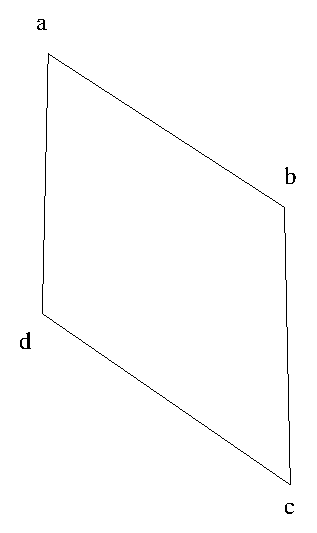
\includegraphics[width=1.0\lengthfigure]{interface.eps}
\caption{Face at the interface defined by the points $\vec{a}$, $\vec{b}$, $\vec{c}$, and $\vec{d}$.}
\label{fig:interface}
\end{figure}


As shown in Fig.\ \ref{fig:interface}, consider a face between two nodes defined by the 4 coordinates $(a_x,~a_y,~a_z)$, $(b_x,~b_y,~b_z)$, $(c_x,~c_y,~c_z)$, and $(d_x,~d_y,~d_z)$.  Define the vectors $\vec{ca}$ and $\vec{ba}$ as:
%
\begin{equation}
\vec{ba}=\vec{b}-\vec{a}
\end{equation}
%
%
\begin{equation}
\vec{ca}=\vec{c}-\vec{a}
\end{equation}
%
Then the cross product between these two vectors is:
%
\begin{equation}
\vec{g}=\vec{ba} \times \vec{ca}
\end{equation}
%
or
%
\begin{equation}
\vec{g}=\left|\begin{array}{ccc} 
\vec{i} & \vec{j} & \vec{k} \\
\vec{ba}_x & \vec{ba}_y & \vec{ba}_z \\
\vec{ca}_x & \vec{ca}_y & \vec{ca}_z 
\end{array}   \right|
\end{equation}
%
or
%
\begin{equation}
\vec{g}=
   (\vec{ba}_y \vec{ca}_z-  \vec{ba}_z \vec{ca}_y)\vec{i}
 + (\vec{ba}_z \vec{ca}_x - \vec{ca}_z \vec{ba}_x)\vec{j}
 + (\vec{ba}_x \vec{ca}_y - \vec{ba}_y \vec{ca}_x)\vec{k}
\end{equation}
%
From the cross product, we can find find the area of the triangle
%
\begin{equation}
A=\frac{1}{2}\sqrt{
   \vec{g}_x^2
 + \vec{g}_y^2
 + \vec{g}_z^2
  }
\end{equation}
%
and we can find the unit normal vector as (i.e.\ vector normal to the triangle):
%
\begin{equation}
\vec{n}=\frac{1}{2A}\left(\vec{g}_x\vec{i}+\vec{g}_y\vec{j} + \vec{g}_z\vec{k}\right)
\end{equation}
%
But what we need is the multiplication between $\vec{n}$ and $A$ which we will denote as $\vec{abc}$:
%
\begin{equation}
\vec{abc}=A\vec{n}=\frac{1}{2}\left(\vec{g}_x\vec{i}+\vec{g}_y\vec{j} + \vec{g}_z\vec{k}\right)
\end{equation}
%
or
%
\begin{equation}
\vec{abc}=\frac{\vec{ba}_y \vec{ca}_z-  \vec{ba}_z \vec{ca}_y}{2}\vec{i}+\frac{\vec{ba}_z \vec{ca}_x - \vec{ca}_z \vec{ba}_x}{2}\vec{j} + \frac{\vec{ba}_x \vec{ca}_y - \vec{ba}_y \vec{ca}_x}{2}\vec{k}
\end{equation}
%

The vector $\vec{abc}$ is not unique as it can point in two directions. To verify that it points in the right direction, calculate the dot product between $\vec{abc}$ and a vector linking the two nodes adjacent to the interface. If the dot product is positive then $\vec{abc}$ points in the right direction. If not, then change the sign of each component of $\vec{abc}$.  

Following similar steps, we can find the vector associated with the second triangle part of the face with the corners located at $\vec{a}$, $\vec{d}$ and $\vec{c}$:
%
\begin{equation}
\vec{adc}=\frac{\vec{da}_y \vec{ca}_z-  \vec{da}_z \vec{ca}_y}{2}\vec{i}+\frac{\vec{da}_z \vec{ca}_x - \vec{ca}_z \vec{da}_x}{2}\vec{j} + \frac{\vec{da}_x \vec{ca}_y - \vec{da}_y \vec{ca}_x}{2}\vec{k}
\end{equation}
%
Now, at the interface perpendicular to the dimension $\theta$, 
%
\begin{equation}
\Omega X_{\theta,j}= \vec{abc}_j + \vec{adc}_j
\end{equation}
%
Or
%
\begin{equation}
X_{\theta,j}= \frac{\vec{abc}_j + \vec{adc}_j}{\Omega }
\end{equation}
%



  \bibliographystyle{warpdoc}
  \bibliography{all}



\end{document}









